\documentclass[11pt]{article}
\usepackage{float}
\usepackage[utf8]{inputenc}
\usepackage[T1]{fontenc}
\usepackage[brazilian]{babel}
\usepackage{graphicx}
\usepackage{booktabs}
\usepackage{amsmath}
\usepackage{amssymb}
\usepackage{hyperref}
\usepackage[a4paper,margin=1.8cm,top=1.7cm,bottom=1.7cm]{geometry}
\usepackage{enumitem}
\setlist{noitemsep, topsep=2pt, parsep=0pt}
\usepackage{setspace}
\usepackage{subcaption}
\usepackage{helvet}
\renewcommand{\familydefault}{\sfdefault}
\setstretch{1.15}


\title{Modelagem, Implementação e Análise Comparativa de\\
Estruturas em Árvore Especializadas}
\author{Carlos Daniel Barbosa Silveira \\ Algoritmos e Estruturas de Dados II \\ Professor: Michel Pires da Silva \\ CEFET-MG}
\date{Setembro de 2026}

\begin{document}
\maketitle

\begin{abstract}
Este trabalho apresenta o estudo, a implementação e a análise comparativa de cinco
estruturas de dados hierárquicas especializadas -- Trie, Árvore Patricia, Árvore
Splay, Árvore Treap e KD-Tree -- em contraste com as estruturas fundamentais de
Árvore Binária de Busca (BST) e Árvore AVL. São discutidos os fundamentos teóricos,
as decisões de projeto adotadas na implementação em C++, a análise de complexidade
assintótica e os resultados de experimentos computacionais que avaliam o
comportamento prático de cada estrutura sob diferentes cargas de dados. O código-fonte
completo, os scripts de experimento e as representações visuais geradas encontram-se
disponíveis no repositório do projeto no GitHub.
\end{abstract}

\vspace{0.5cm}
\tableofcontents

\newpage

% =========================================================
\section{Introdução e Fundamentação Teórica}
% =========================================================

\subsection{Contextualização e Motivação}

Estruturas de dados hierárquicas organizam e recuperam informação de forma
eficiente. BST e AVL oferecem uma solução geral para chaves comparáveis, com
custo logarítmico de busca, inserção e remoção -- mas essa generalidade não
explora características específicas dos dados, como compartilhamento de
prefixos entre strings, padrões de acesso desiguais ao longo do tempo, ou a
natureza multidimensional de certos conjuntos de dados. Este trabalho investiga
cinco estruturas especializadas, cada uma motivada por uma limitação distinta
das árvores genéricas:

\begin{itemize}
    \item \textbf{Trie} e \textbf{Patricia}: ineficiência de uma BST ao
    armazenar strings com prefixos compartilhados, já que ela compara strings
    inteiras a cada nó, sem reaproveitar prefixos comuns.
    \item \textbf{Splay}: padrões de acesso não uniformes, em que poucos
    elementos são consultados com muito mais frequência (localidade temporal).
    \item \textbf{Treap}: complexidade de implementação de árvores balanceadas
    por regras determinísticas (AVL), propondo balanceamento probabilístico.
    \item \textbf{KD-Tree}: necessidade de organizar pontos multidimensionais,
    problema para o qual uma BST unidimensional não se aplica.
\end{itemize}

\subsection{Trie (Árvore de Prefixos)}

Cada aresta representa um único caractere, e o caminho da raiz até um nó
representa o prefixo formado pela concatenação desses caracteres (a raiz
representa a string vazia).
\textbf{Nó:} vetor de até 26 ponteiros (um por letra), permitindo acesso ao
filho em tempo constante, e um booleano indicando fim de palavra.
\textbf{Invariante:} cada nível representa um caractere adicional da chave;
palavras com prefixos comuns compartilham o mesmo caminho até divergirem.

\subsection{Árvore Patricia (Radix Tree Compacta)}

Resolve uma ineficiência estrutural da Trie: sequências de nós sem ramificação
(um único filho), que ocorrem quando um trecho da chave não diverge de nenhuma
outra. A Patricia comprime esses ``corredores'' em uma única aresta rotulada
com a substring inteira.
\textbf{Nó:} rótulo (\texttt{std::string}) do trecho comprimido, vetor de
filhos indexado pela primeira letra do restante da chave, e fim de palavra.
\textbf{Invariante:} todo nó interno que não seja fim de palavra deve possuir
pelo menos dois filhos -- caso contrário representaria um corredor sem
ramificação, que deveria estar comprimido com seu único filho.

\subsection{Árvore Splay}

BST autoajustável: toda operação de acesso desloca o nó acessado até a raiz
por rotações. Três padrões: \textit{zig} (nó filho direto da raiz),
\textit{zig-zig} (nó e pai do mesmo lado em relação ao avô) e \textit{zig-zag}
(lados opostos).
\textbf{Nó:} chave, ponteiros para filho esquerdo, direito e \textbf{pai} --
necessário para determinar a relação com pai/avô durante a reorganização sem
busca adicional.
\textbf{Invariante:} a propriedade de BST é mantida sempre; não há invariante
de balanceamento estrutural formal -- o desempenho é garantido apenas de forma
\textit{amortizada} ao longo de uma sequência de operações.

\subsection{Árvore Treap}

Combina BST (ordenação por chave) com heap (ordenação por prioridade). Cada
nó recebe, ao ser criado, uma prioridade aleatória.
\textbf{Nó:} chave, prioridade (inteiro aleatório), filho esquerdo e direito.
\textbf{Invariante:} a prioridade de todo nó é maior ou igual à de seus
filhos. Como as prioridades são independentes da ordem de inserção, o formato
resultante equivale, em distribuição, ao de uma BST construída por inserção
aleatória -- altura esperada $O(\log n)$.

\subsection{KD-Tree}

Generaliza a BST para espaços multidimensionais, alternando a dimensão de
comparação a cada nível: profundidade par compara $x$, ímpar compara $y$.
\textbf{Nó:} coordenadas do ponto ($x$, $y$), filho esquerdo e direito.
\textbf{Invariante:} a cada nível, o subespaço é particionado por um
hiperplano perpendicular ao eixo daquele nível -- pontos ``menores'' à
esquerda, ``maiores'' à direita.

\subsection{Síntese comparativa com BST e AVL}

A diferença conceitual central é que BST/AVL são estruturas de propósito
geral, com desempenho dependente apenas de $n$; Trie e Patricia dependem do
\textbf{comprimento da chave} ($L$), independentemente de $n$; Splay explora
\textbf{padrões de acesso} ao longo do tempo; Treap alcança balanceamento
\textbf{probabilístico} em vez de determinístico; e a KD-Tree estende o
conceito de BST para \textbf{múltiplas dimensões}.

% =========================================================
\section{Projeto e Implementação das Estruturas}
% =========================================================

Esta seção descreve as decisões de projeto adotadas na implementação em C++ de
cada estrutura. O código completo está disponível no repositório do projeto; o
conteúdo aqui apresentado limita-se aos trechos essenciais para explicar
mecanismos e decisões relevantes.

\subsection{Trie}

O nó foi representado por um vetor fixo \texttt{NoTrie* filhos[26]} e um
booleano \texttt{fimDePalavra}. A decisão de utilizar vetor fixo, em vez de
\texttt{unordered\_map<char, NoTrie*>}, favorece a previsibilidade da análise
assintótica: acesso a um filho é $O(1)$ constante e determinístico, facilitando
a justificativa formal de complexidade (Seção 4); a desvantagem -- maior
consumo de memória em conjuntos esparsos -- é discutida na Seção 6.

A remoção (\texttt{removerAux}) é a operação mais sutil: um nó só pode ser
fisicamente removido se não for mais fim de palavra \textbf{e} não possuir
filhos. A função é recursiva, descendo até o fim da palavra e, na volta,
verificando em cada nível se o nó tornou-se desnecessário, propagando a
decisão ao nível superior.

\subsection{Patricia}

O nó adiciona, em relação à Trie, um rótulo \texttt{std::string rotulo},
permitindo que uma aresta represente múltiplos caracteres. A inserção trata
três casos: (a) o rótulo do filho corresponde integralmente ao trecho da
chave, bastando descer e continuar com o restante; (b) não existe filho para a
primeira letra do restante, criando-se um nó novo; e (c) o rótulo diverge no
meio, exigindo um nó intermediário que particiona o rótulo original em duas
partes -- o caso mais complexo, pois o nó original (com seus filhos e estado
de fim de palavra) deve ser preservado, apenas com o rótulo reduzido.

\subsection{Splay}

O nó inclui um ponteiro adicional para o pai, essencial para que a
reorganização (\texttt{splay}) determine a relação com pai/avô sem busca
adicional. As rotações foram implementadas como duas funções simétricas
(\texttt{rotacionarDir}/\texttt{rotacionarEsq}), parametrizadas pelo nó que
desce. A distinção em relação a uma dupla rotação de AVL está na ordem do caso
\textit{zig-zig}: a rotação é aplicada primeiro sobre o avô e depois sobre o
pai -- e não o inverso --, o que caracteriza o autoajuste da Splay.

A remoção usa a técnica de \textit{join}: após trazer o nó a remover até a
raiz, sua subárvore esquerda e direita são separadas; o maior elemento da
subárvore esquerda é deslocado ao topo (via \texttt{splay}), garantindo
ausência de filho direito, permitindo anexar a subárvore direita original.

\subsection{Treap}

As rotações retornam a nova raiz da subárvore, sem exigir ponteiro para o pai
-- a recursão natural já mantém o contexto necessário. A inserção segue o
comportamento padrão de BST e, ao retornar da recursão, corrige violações da
propriedade de heap (filho com prioridade maior que o pai) via rotação. A
remoção de um nó com dois filhos gira, a cada passo, o filho de maior
prioridade para cima, empurrando o nó a remover até possuir zero ou um filho.

\subsection{KD-Tree}

A alternância de dimensão de comparação é implementada através de um parâmetro
de profundidade, propagado recursivamente: profundidade par compara a
coordenada $x$, profundidade ímpar compara $y$. A escolha de alternar
estritamente por paridade de profundidade (em vez de escolher a dimensão de
maior variância, uma otimização possível) foi feita em favor da simplicidade
de implementação, sendo essa uma limitação discutida na Seção 6.

A remoção é a operação mais sutil da KD-Tree, por não admitir a estratégia
clássica de BST de substituir o nó removido pelo mínimo da subárvore
direita indiscriminadamente: o substituto precisa ser, especificamente, o
ponto de \emph{menor valor na dimensão de corte daquele nível} -- pois um
ponto com menor valor em outra dimensão poderia, ainda assim, violar o
invariante de particionamento. Quando o nó a remover não possui subárvore
direita, o algoritmo busca o mínimo na subárvore \emph{esquerda} e a
reatribui inteira como nova subárvore direita, já que, após a substituição,
todos os pontos remanescentes possuem valor maior ou igual ao novo nó
naquela dimensão -- convenção adotada também na inserção.

\subsection{Visualização (comum às cinco estruturas)}

Todas as estruturas implementam um método \texttt{exportarDot}, que percorre a
árvore recursivamente e gera um arquivo no formato Graphviz (\texttt{.dot}),
posteriormente renderizado em SVG. Essa abordagem desacopla completamente a
lógica da estrutura de dados da lógica de renderização.

% =========================================================
\section{Demonstração e Rastreamento Visual}

Esta seção apresenta a evolução topológica das cinco estruturas estudadas, demonstrando os estados inicial, intermediário (bifurcação, rotação ou autoajuste) e pós-remoção por meio de representações extraídas diretamente da memória via \texttt{exportarDot} e convertidas em imagens de alta definição.

\subsection{Trie e Árvore Patricia: Compactação de Prefixos}

A Figura~\ref{fig:trie_patricia_comp} confronta a organização da Trie com a compactação realizada pela Patricia sobre o mesmo conjunto de termos (\texttt{"casa"}, \texttt{"casal"}, \texttt{"casamento"}, \texttt{"casarão"}).

\begin{figure}[H]
    \centering
    \begin{subfigure}[b]{0.48\textwidth}
        \centering
        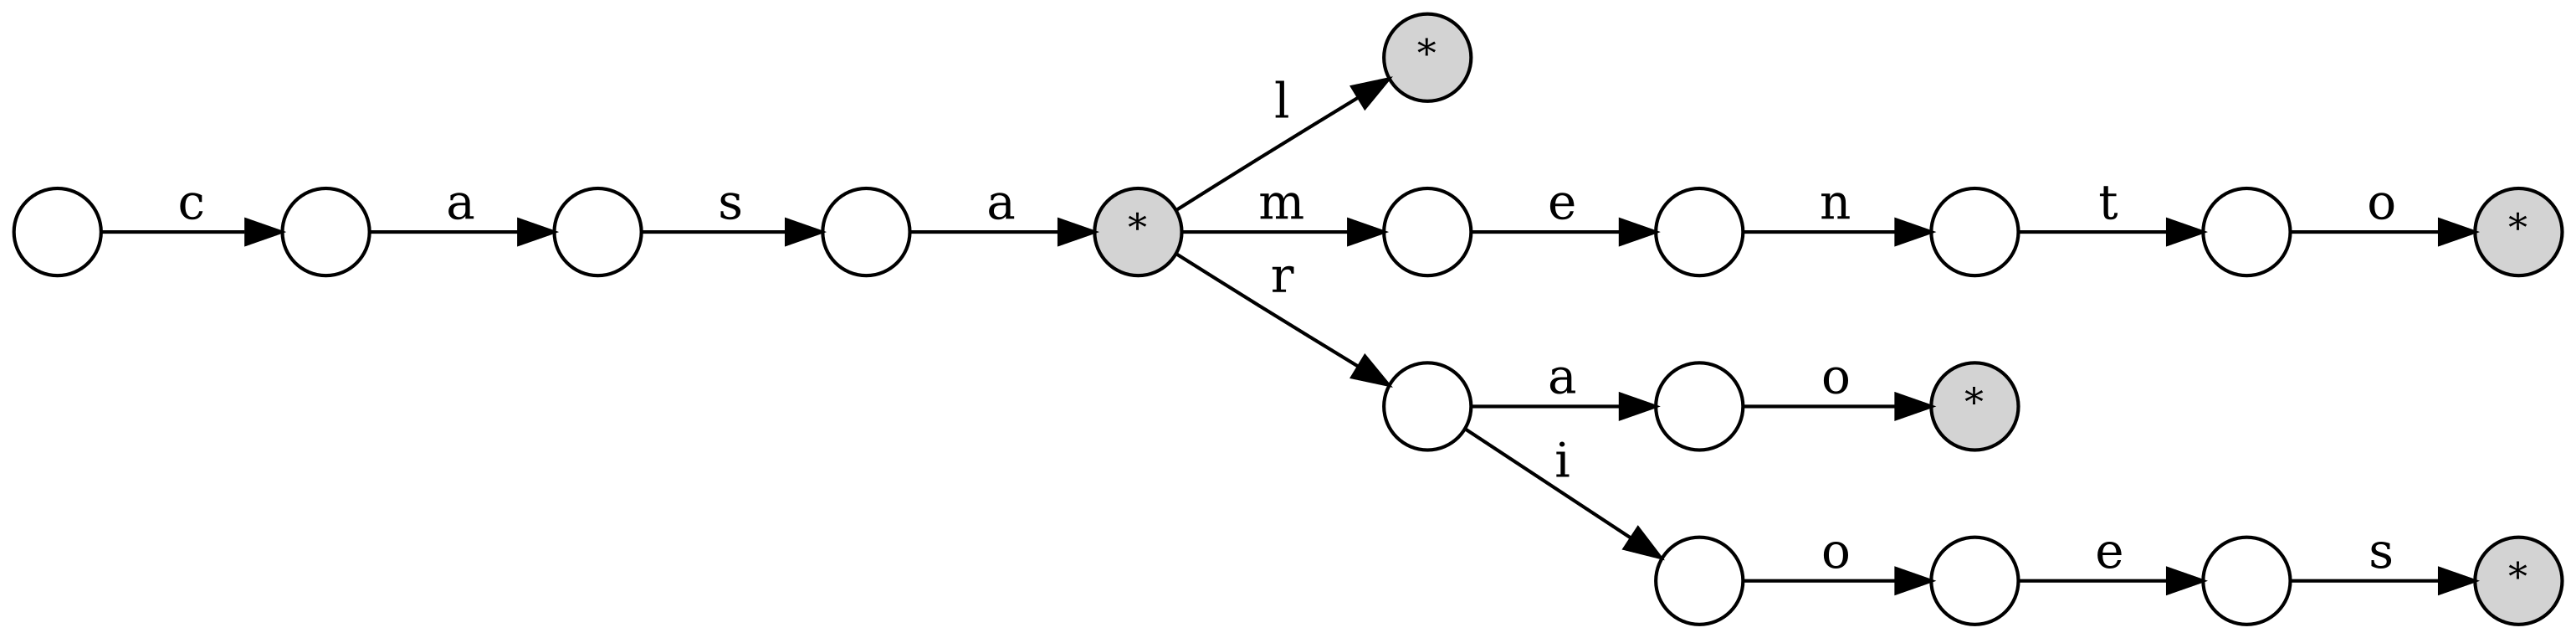
\includegraphics[width=\linewidth, height=3.8cm, keepaspectratio]{figuras/trie_2_ramificacao.png}
        \caption{Trie: cadeias unárias explícitas.}
        \label{fig:trie_vis}
    \end{subfigure}
    \hfill
    \begin{subfigure}[b]{0.48\textwidth}
        \centering
        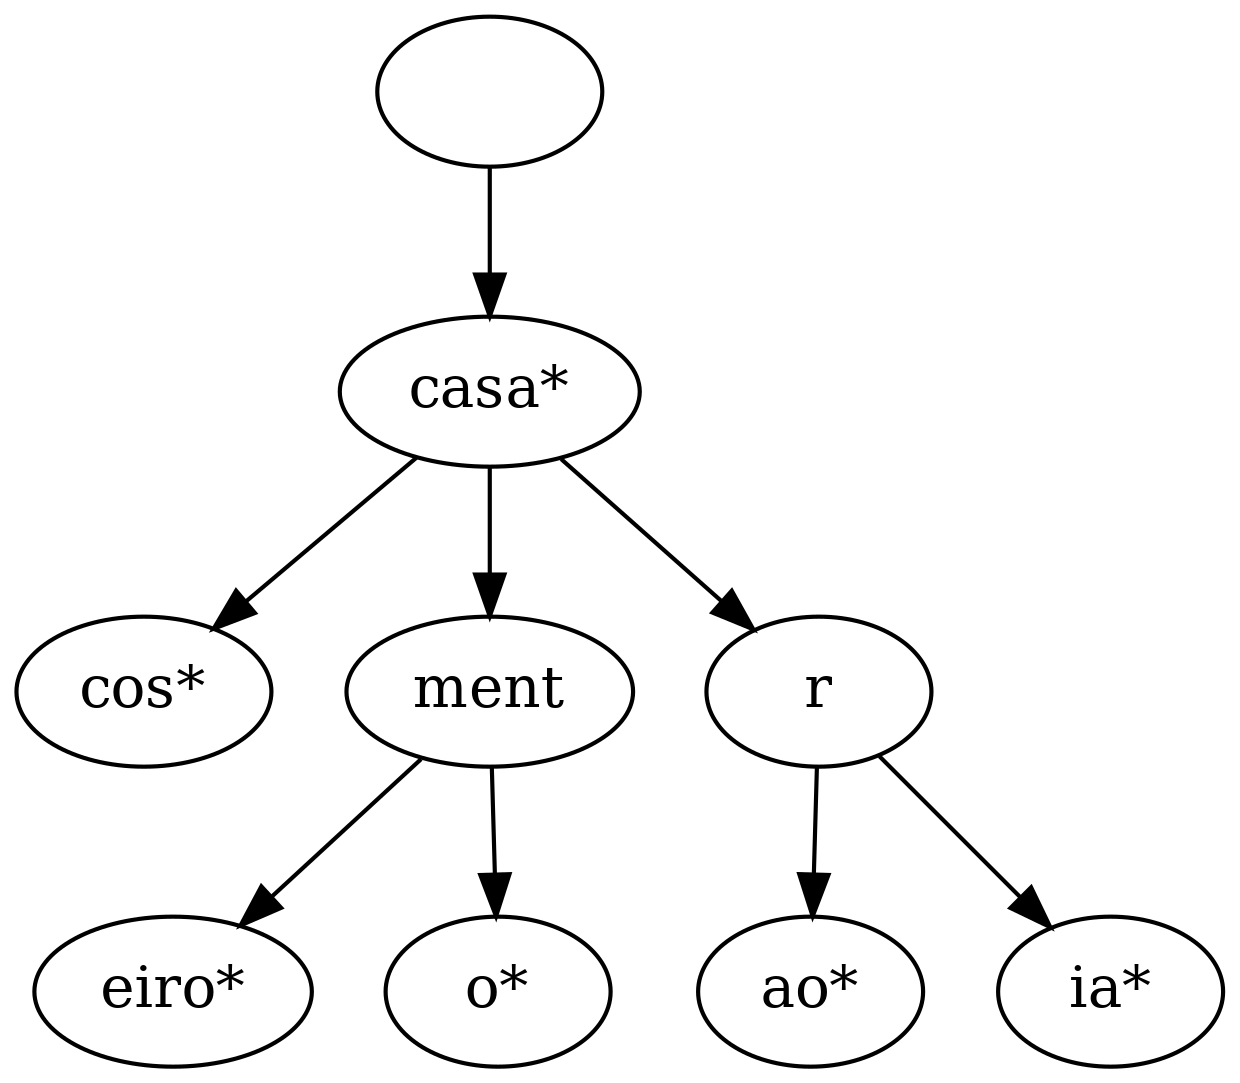
\includegraphics[width=\linewidth, height=3.8cm, keepaspectratio]{figuras/patricia_2_divisao.png}
        \caption{Patricia: arestas comprimidas.}
        \label{fig:patricia_vis}
    \end{subfigure}
    \caption{Comparativo visual: eliminação de corredores unários e divisão de rótulos (\textit{edge split}) na Patricia.}
    \label{fig:trie_patricia_comp}
\end{figure}

Na Trie (Figura~\ref{fig:trie_vis}), cada caractere exige um nó dedicado, gerando cadeias lineares para sufixos sem bifurcação. Na Patricia (Figura~\ref{fig:patricia_vis}), sequências de nós com grau de saída 1 são condensadas em arestas únicas contendo substrings inteiras. Ao inserir termos divergentes, a Patricia realiza o corte seletivo do rótulo (\textit{split}), mantendo a invariante de que nós internos não terminais possuem grau $\ge 2$.

\subsection{Árvore Splay: Autoajuste via Rotações}

A Figura~\ref{fig:splay_comp} ilustra a reestruturação topológica promovida pela operação de \textit{splay} ao acessar uma chave profunda.

\begin{figure}[H]
    \centering
    \begin{subfigure}[b]{0.48\textwidth}
        \centering
        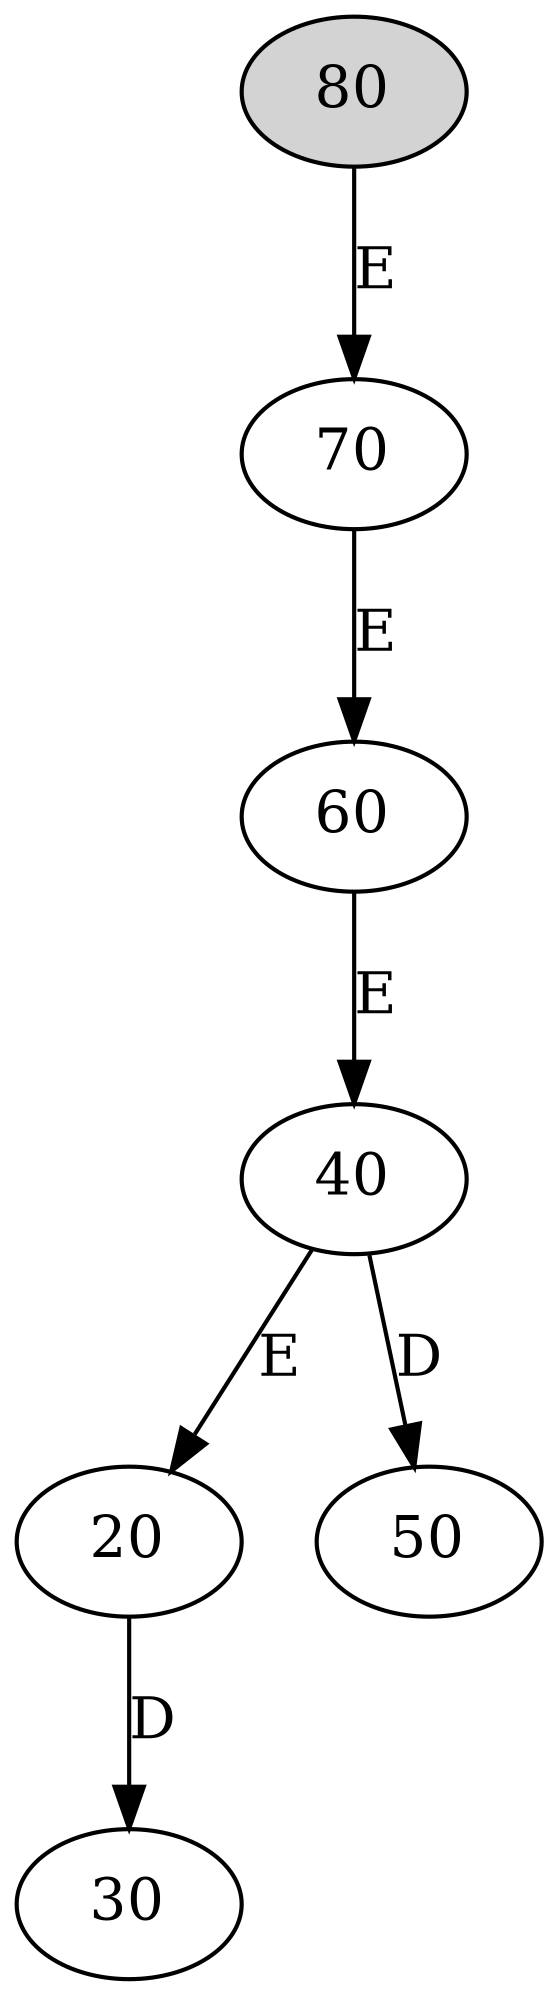
\includegraphics[width=\linewidth, height=3.8cm, keepaspectratio]{figuras/splay_1_inicial.png}
        \caption{Estado inicial antes da consulta.}
        \label{fig:splay_ini}
    \end{subfigure}
    \hfill
    \begin{subfigure}[b]{0.48\textwidth}
        \centering
        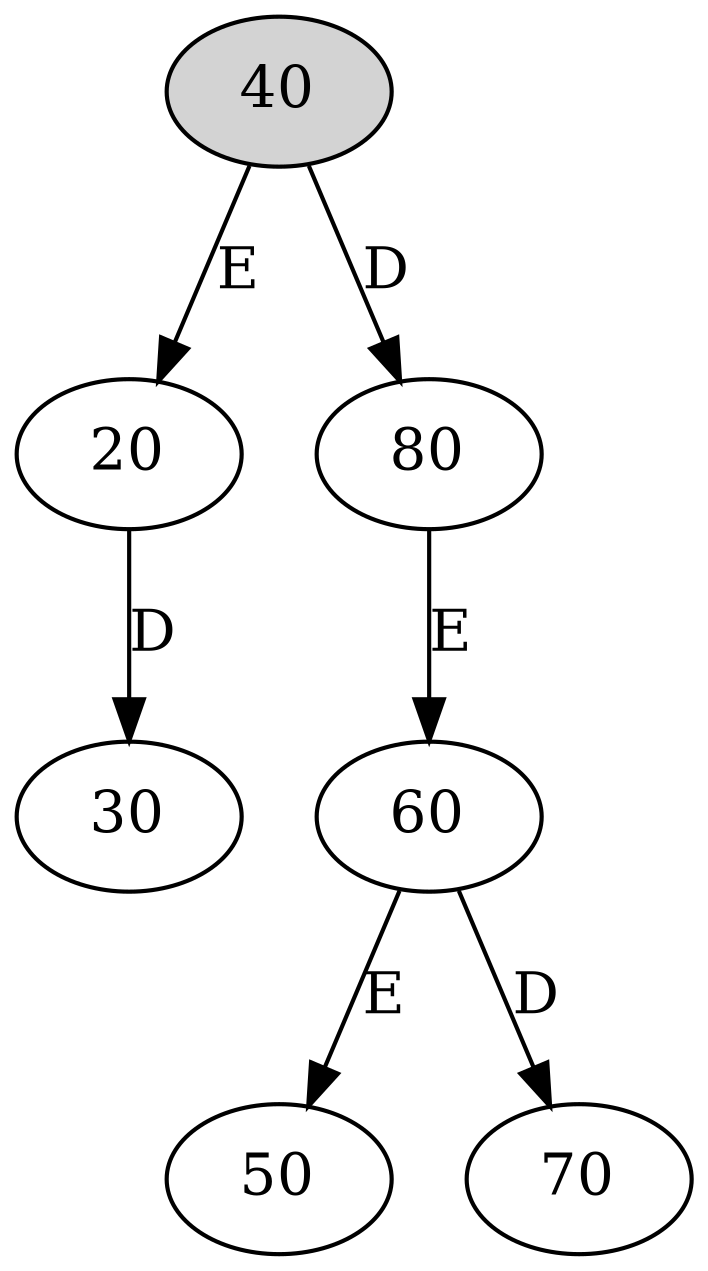
\includegraphics[width=\linewidth, height=3.8cm, keepaspectratio]{figuras/splay_2_apos_splay_de_40.png}
        \caption{Após \textit{splay}: nó elevado à raiz.}
        \label{fig:splay_fim}
    \end{subfigure}
    \caption{Reorganização da Splay: aplicação de passos \textit{zig-zig} e \textit{zig-zag} reduzindo a profundidade média da árvore.}
    \label{fig:splay_comp}
\end{figure}

O acesso a uma chave em nó folha dispara rotações compostas que transportam o elemento acessado até a raiz (Figura~\ref{fig:splay_fim}). Esse processo diminui pela metade a distância dos nós ao longo do caminho de busca, garantindo custo amortizado logarítmico e favorecendo acessos com forte localidade temporal.

\subsection{Árvore Treap e KD-Tree}

A Figura~\ref{fig:treap_kdtree_comp} exibe a dupla invariante da Treap e a partição alternada de eixos na KD-Tree.

\begin{figure}[H]
    \centering
    \begin{subfigure}[b]{0.48\textwidth}
        \centering
        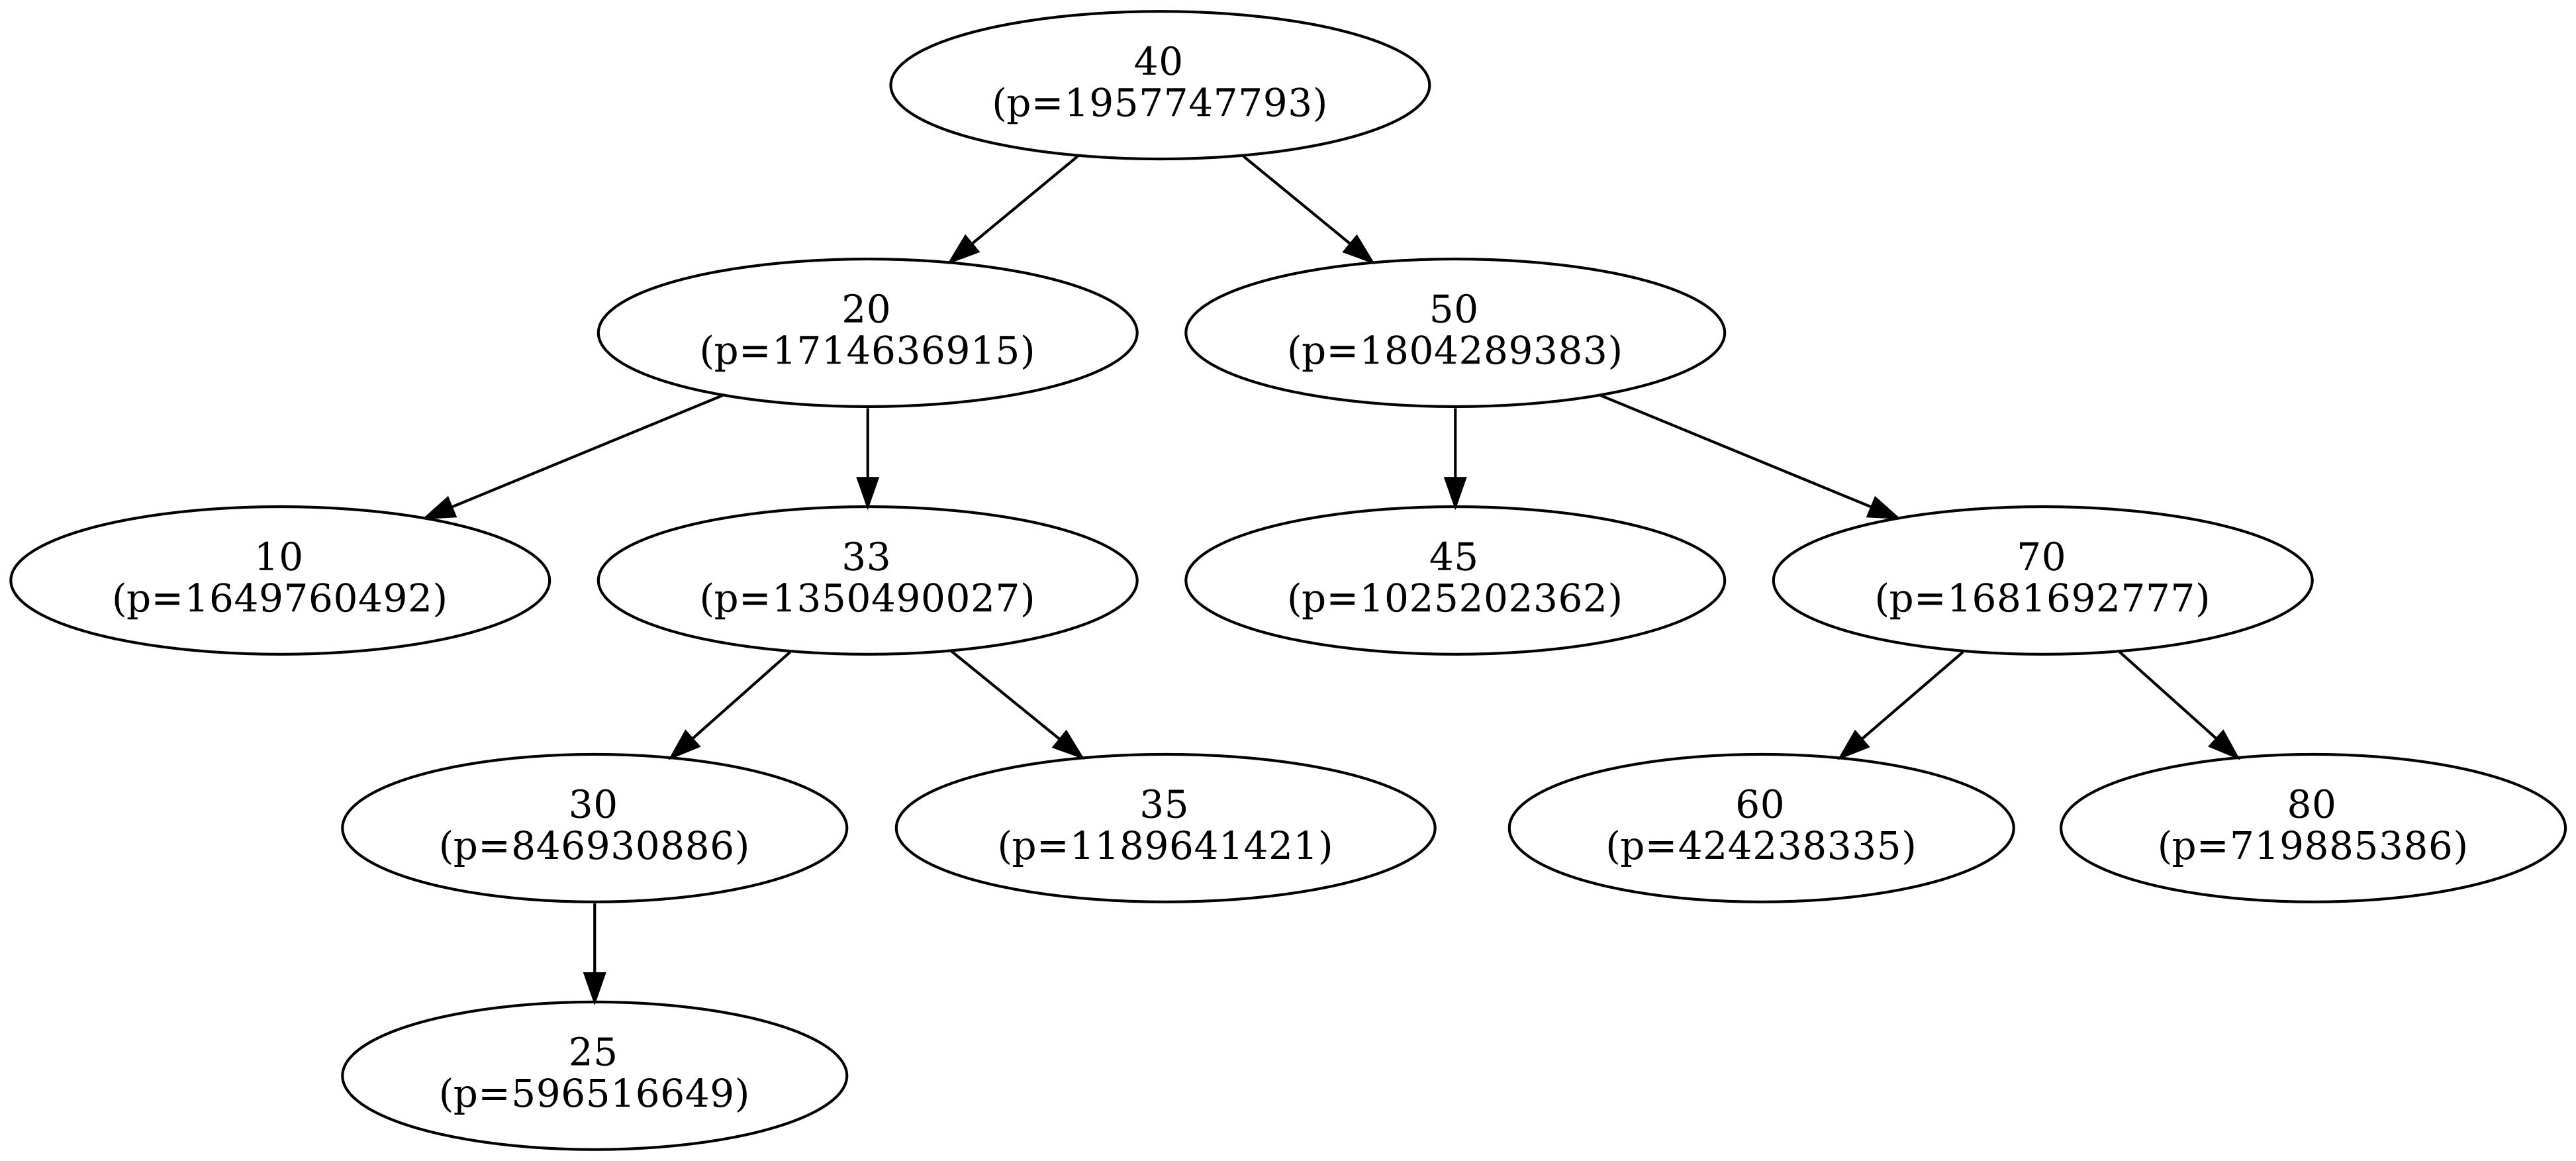
\includegraphics[width=\linewidth, height=3.8cm, keepaspectratio]{figuras/treap_2_pos_insercao.png}
        \caption{Treap: tuplas \texttt{chave (prioridade)}.}
        \label{fig:treap_vis}
    \end{subfigure}
    \hfill
    \begin{subfigure}[b]{0.48\textwidth}
        \centering
        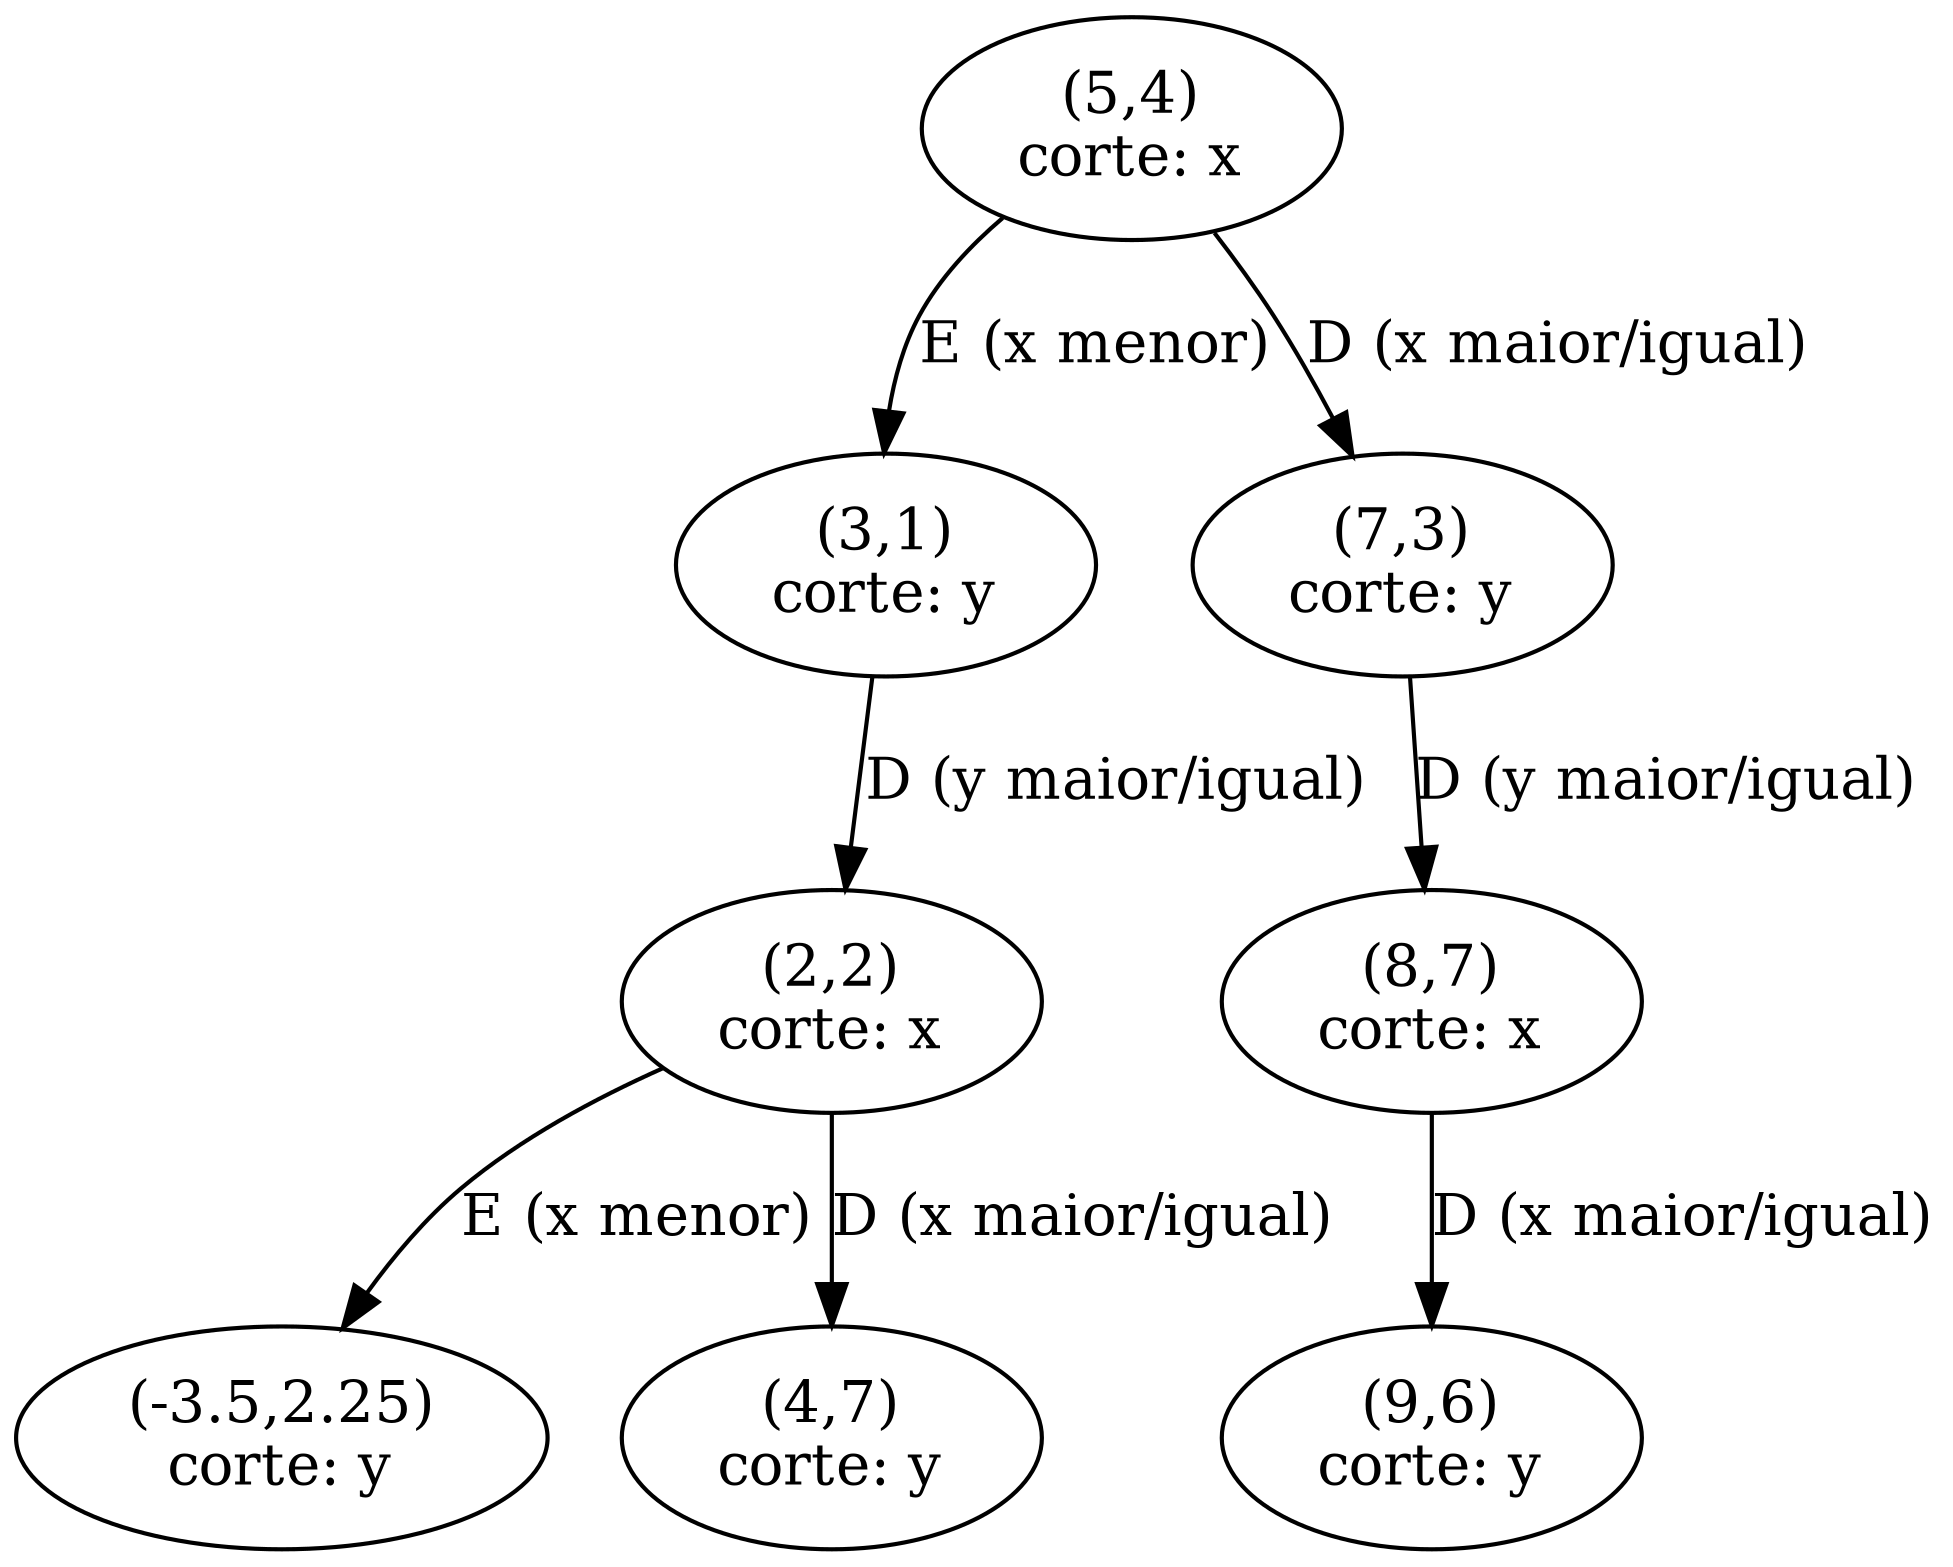
\includegraphics[width=\linewidth, height=3.8cm, keepaspectratio]{figuras/kdtree_2_pos_insercao.png}
        \caption{KD-Tree: partição ortogonal de eixos.}
        \label{fig:kdtree_vis}
    \end{subfigure}
    \caption{Estruturas especializadas: (a) Treap balanceada via prioridades aleatórias; (b) KD-Tree particionando o espaço $\mathbb{R}^2$.}
    \label{fig:treap_kdtree_comp}
\end{figure}

Mesmo recebendo chaves ordenadas, a Treap (Figura~\ref{fig:treap_vis}) utiliza rotações locais sempre que uma nova prioridade aleatória supera a de seu pai, garantindo altura esperada $O(\log n)$. Na KD-Tree (Figura~\ref{fig:kdtree_vis}), a alternância dos eixos ($X$ nos níveis pares e $Y$ nos ímpares) divide o plano em células retangulares delimitadoras, permitindo a poda euclidiana de ramos inteiros durante consultas por vizinho mais próximo.
% =========================================================
\section{Análise de Complexidade e Comparação Teórica}
% =========================================================

\subsection{Tabela comparativa de complexidade assintótica}

Na tabela a seguir, $n$ representa o número de chaves armazenadas e $L$
representa o comprimento médio de uma chave (aplicável apenas a Trie e
Patricia).

\begin{table}[htbp]
\centering
\renewcommand{\arraystretch}{1.5}
\setlength{\tabcolsep}{10pt}
\resizebox{\textwidth}{!}{%
\begin{tabular}{lccccc}
\toprule
\textbf{Estrutura} & \textbf{Busca} & \textbf{Inserção} & \textbf{Remoção} & \textbf{Construção} & \textbf{Espaço} \\
\midrule
BST (pior caso) & $O(n)$ & $O(n)$ & $O(n)$ & $O(n^2)$ & $O(n)$ \\
BST (caso médio) & $O(\log n)$ & $O(\log n)$ & $O(\log n)$ & $O(n \log n)$ & $O(n)$ \\
AVL & $O(\log n)$ & $O(\log n)$ & $O(\log n)$ & $O(n \log n)$ & $O(n)$ \\
Trie & $O(L)$ & $O(L)$ & $O(L)$ & $O(nL)$ & $O(nL \cdot |\Sigma|)$ \\
Patricia & $O(L)$ & $O(L)$ & $O(L)$ & $O(nL)$ & $O(n \cdot |\Sigma|)$ \\
Splay (amortizado) & $O(\log n)$ & $O(\log n)$ & $O(\log n)$ & $O(n \log n)$ & $O(n)$ \\
Splay (pior caso único) & $O(n)$ & $O(n)$ & $O(n)$ & -- & $O(n)$ \\
Treap (esperado) & $O(\log n)$ & $O(\log n)$ & $O(\log n)$ & $O(n \log n)$ & $O(n)$ \\
KD-Tree (balanceada) & $O(\log n)$ & $O(\log n)$ & $O(\sqrt{n})^*$ & $O(n \log n)$ & $O(n)$ \\
\bottomrule
\end{tabular}%
}
\caption{Complexidade assintótica das operações fundamentais. $|\Sigma|$ denota o tamanho do alfabeto (26, neste trabalho). Para a KD-Tree em $\mathbb{R}^2$, a remoção possui custo médio $O(\log n)$ via localização recursiva do nó sucessor/mínimo no discriminador correspondente (a complexidade $O(\sqrt{n})$ aplica-se a consultas por faixa ortogonal).}
\label{tab:complexidade}
\end{table}

\subsection{Discussão analítica}

\textbf{Trie e Patricia dependem de $L$, não de $n$:} em ambas, o número de
comparações em uma busca ou inserção é, no máximo, o comprimento da chave --
a árvore nunca é percorrida mais fundo que o tamanho da própria chave,
independentemente de $n$. Comportamento investigado na Seção 5.

\textbf{Patricia usa menos espaço:} ao comprimir sequências de nós sem
ramificação em um único nó com rótulo de múltiplos caracteres, elimina
exatamente os nós que, na Trie, existiriam só para representar uma letra sem
alternativa. Quanto mais exclusivo o sufixo de uma chave, maior a economia.

\textbf{Splay tem garantia apenas amortizada:} uma operação isolada pode
custar $O(n)$ (ex.: acessar o elemento mais profundo de uma árvore
momentaneamente degenerada), mas o \textit{splay} subsequente reorganiza a
árvore para beneficiar operações futuras -- ao longo de $m$ operações, o
custo total é $O(m \log n)$.

\textbf{Treap tem apenas garantia esperada:} como as prioridades são
aleatórias, existe probabilidade (exponencialmente pequena) de uma sequência
degenerada -- desprezível na prática, mas sem a garantia de pior caso da AVL.

\textbf{Comparação com BST e AVL:} a AVL garante $O(\log n)$ via rotações
determinísticas com maior custo de implementação. A Treap alcança garantia
probabilisticamente equivalente com implementação mais simples. A Splay não
busca balanceamento estrutural -- sua vantagem está no comportamento agregado
sob acesso não uniforme, cenário para o qual BST/AVL não oferecem vantagem.

% =========================================================
\section{Metodologia Experimental e Resultados}
% =========================================================

\subsection{Metodologia}

Os experimentos foram implementados em C++, com medição de tempo via
\texttt{std::chrono} (relógio de alta resolução), e conduzidos com semente
fixa (\texttt{srand(42)}) para garantir reprodutibilidade. Os tamanhos de
entrada avaliados foram $n \in \{10, 10^3, 10^4, 10^5\}$.

\textbf{Trie e Patricia:} avaliadas sobre três conjuntos de palavras aleatórias
de comprimento fixo -- ``curto'' (3 caracteres), ``médio'' (8 caracteres) e
``longo'' (20 caracteres) --, operacionalizando os conceitos de melhor, médio e
pior caso discutidos na Seção 4 em termos do comprimento da chave, e não da
quantidade de chaves.

\textbf{Splay e Treap:} avaliadas sobre dois padrões de inserção -- chaves em
ordem aleatória e chaves em ordem estritamente crescente --, o segundo sendo o
caso clássico de degeneração de uma BST não balanceada. Um experimento
adicional avaliou o efeito da localidade de acesso, comparando um padrão de
acesso enviesado (80\% das operações concentradas em 20\% das chaves) contra um
padrão uniforme.

\textbf{KD-Tree:} avaliada sobre um conjunto de pontos bidimensionais gerados
aleatoriamente, medindo inserção, busca e remoção.


\subsection{Resultados: Trie vs. Patricia}

\begin{figure}[H]
    \centering
    
\includegraphics[width=0.95\textwidth]{figuras/01_insercao_trie_vs_patricia.png}
    \caption{Tempo de inserção: Trie vs. Patricia (casos curto, médio e longo).}
    \label{fig:insercao_trie_patricia}
\end{figure}

\begin{figure}[H]
    \centering
    
\includegraphics[width=0.95\textwidth]{figuras/02_busca_trie_vs_patricia.png}
    \caption{Tempo de busca: Trie vs. Patricia (casos curto, médio e longo).}
    \label{fig:busca_trie_patricia}
\end{figure}

\begin{figure}[H]
    \centering
    
\includegraphics[width=0.62\textwidth]{figuras/03_memoria_trie_vs_patricia.png}
    \caption{Número de nós e memória estimada, Trie vs. Patricia ($n=1000$).}
    \label{fig:memoria_trie_patricia}
\end{figure}

Os resultados (Figura~\ref{fig:insercao_trie_patricia}) confirmam a previsão
teórica de forma marcante: no caso ``longo'', a Trie cresce de forma muito mais
acentuada que a Patricia à medida que $n$ aumenta -- a diferença de tempo de
inserção em $n=10^5$ é de aproximadamente 5,6 vezes (Trie mais lenta). No caso
``curto'', por outro lado, a Trie é ligeiramente mais rápida que a Patricia em
todos os tamanhos testados, evidenciando que a compressão de rótulos da
Patricia introduz um sobrecusto (manipulação de \texttt{std::string},
comparação de substrings) que só compensa quando as chaves são
suficientemente longas para que a economia estrutural supere esse sobrecusto.

O tempo de busca (Figura~\ref{fig:busca_trie_patricia}) apresenta um padrão
análogo, porém com o cruzamento entre as duas estruturas ocorrendo em pontos
distintos conforme o comprimento da chave -- no caso ``longo'', a Patricia
supera a Trie a partir de valores intermediários de $n$.

A Figura~\ref{fig:memoria_trie_patricia} evidencia diretamente o mecanismo
responsável por essas diferenças: para chaves longas, a Trie utilizada
aproximadamente 14 vezes mais nós que a Patricia para representar o mesmo
conjunto de 1000 chaves, confirmando experimentalmente a economia de espaço
discutida teoricamente na Seção 4.

\subsection{Resultados: Splay vs. Treap}

\begin{figure}[htbp]
    \centering
    
\includegraphics[width=0.85\textwidth]{figuras/04_splay_treap_aleatorio_vs_ordenado.png}
    \caption{Splay vs. Treap: inserção ordenada de chaves crescentes vs. aleatória.}
    \label{fig:splay-treap}
\end{figure}

Um resultado experimental notável, e à primeira vista contraintuitivo, é
visível na Figura~\ref{fig:splay-treap}: para \emph{ambas} as estruturas, a
inserção em ordem crescente é mais rápida que a aleatória, quando o esperado
seria o oposto (degeneração em lista encadeada). A explicação está no
mecanismo de \textit{splay}: ao inserir chaves crescentes, cada nova chave é
sempre maior que a raiz atual, logo sua posição de inserção é imediatamente
acessível a partir da raiz, e o \textit{splay} subsequente a torna raiz em uma
única rotação \textit{zig}. A árvore resultante é uma cadeia degenerada em
altura, mas o \emph{custo de inserção} permanece $O(1)$ por operação -- um
exemplo de como o comportamento amortizado da Splay diverge da intuição
construída sobre BSTs estáticas.

Para a Treap, a diferença entre os dois padrões de inserção é bem menor,
consistente com a previsão teórica de que o balanceamento probabilístico é
\emph{independente} da ordem de inserção das chaves.

\subsection{Localidade de acesso: Splay vs. Treap}

A Figura~\ref{fig:localidade} (apresentada junto à Figura~\ref{fig:kdtree}, adiante)
isola a propriedade central que motiva a Splay:
sob um padrão de acesso enviesado, em que 80\% dos acessos concentram-se em
apenas 20\% das chaves, o tempo médio por acesso da Splay é sensivelmente menor
que sob um padrão de acesso uniforme, e essa vantagem \emph{aumenta} com o
tamanho da árvore -- exatamente o comportamento esperado da localidade
temporal de referência. A Treap, por não realizar nenhuma reorganização
baseada em histórico de acesso, apresenta tempo médio por acesso praticamente
idêntico sob os dois padrões, como previsto teoricamente.

\subsection{Resultados: KD-Tree}

\begin{figure}[htbp]
    \centering
    \begin{minipage}{0.48\textwidth}
        \centering
        
\includegraphics[width=\textwidth]{figuras/05_kdtree_operacoes.png}
        \caption{Tempo de inserção, busca e remoção da KD-Tree em função de $n$.}
        \label{fig:kdtree}
    \end{minipage}
    \hfill
    \begin{minipage}{0.48\textwidth}
        \centering
        
\includegraphics[width=\textwidth]{figuras/06_localidade_splay_vs_treap.png}
        \caption{Tempo médio por acesso: padrão enviesado (80/20) vs. uniforme.}
        \label{fig:localidade}
    \end{minipage}
\end{figure}

A Figura~\ref{fig:kdtree} mostra que as três operações escalam de forma
semelhante entre si em relação a $n$, com a remoção consistentemente mais
custosa que a busca e a inserção -- coerente com a maior complexidade
algorítmica dessa operação na KD-Tree, discutida na Seção 4.

\subsection{Convergência entre teoria e prática}

De forma geral, os resultados experimentais corroboram a análise teórica da
Seção 4: (i) Trie e Patricia demonstram sensibilidade ao comprimento da chave
que a Patricia mitiga por compressão; (ii) a Treap demonstra estabilidade de
desempenho independentemente da ordem de inserção, validando o balanceamento
probabilístico; (iii) a Splay demonstra vantagem clara sob localidade de
acesso, validando sua motivação teórica central. A principal divergência entre
expectativa ingênua e comportamento observado ocorreu na Splay sob inserção
ordenada, elucidada pela análise do mecanismo de \textit{splay} em si.

% =========================================================
\section{Aplicações, Análise Crítica e Discussão}
% =========================================================

\subsection{Aplicações}

\textbf{Trie:} autocompletar e correção ortográfica, onde a busca por todas as
palavras com um prefixo se beneficia da organização por prefixo compartilhado.
\textbf{Patricia:} tabelas de roteamento IP (prefixo mais longo) e indexação
compacta de grandes dicionários, onde volume e comprimento de chave tornam a
economia de memória significativa.
\textbf{Splay:} caches e estruturas com localidade temporal (ex.: cache de
tradução de páginas), onde símbolos recentes tendem a se repetir.
\textbf{Treap:} estruturas que exigem balanceamento eficiente com
implementação simples, priorizando manutenção do código sobre garantia
absoluta de pior caso.
\textbf{KD-Tree:} sistemas GIS, busca do vizinho mais próximo (k-NN) e
geometria computacional em geral.

\subsection{Vantagens, limitações e divergências entre teoria e prática}

A implementação confirmou um \emph{trade-off} claro entre Trie (simplicidade)
e Patricia (eficiência de espaço), esta última vantajosa principalmente para
chaves longas e/ou grandes volumes -- para conjuntos pequenos de chaves
curtas, a Trie é preferível tanto pela simplicidade quanto pelo desempenho
observado.

A Splay demonstrou a maior dificuldade de implementação, pela necessidade de
manter corretamente o ponteiro para o pai e pela distinção sutil entre os
casos \textit{zig-zig} e \textit{zig-zag} -- um erro na ordem das rotações do
\textit{zig-zig} foi identificado e corrigido durante o desenvolvimento, sem o
qual a estrutura manteria a propriedade de BST, mas não o comportamento
amortizado esperado. A KD-Tree, na implementação apresentada, alterna a
dimensão de comparação estritamente por paridade de profundidade, sem
considerar a distribuição real dos dados -- limitação discutida na literatura.

O caso mais notável de divergência entre expectativa teórica e comportamento
observado foi o desempenho da Splay sob inserção ordenada (Seção 5.3): a
intuição de BST clássica prevê degeneração, mas o autoajuste da Splay produz o
efeito oposto para o \emph{custo de inserção}, ainda que a \emph{altura} da
árvore resultante seja de fato degenerada.

\subsection{Melhorias e extensões possíveis}

Destacam-se: (i) \texttt{unordered\_map} como estrutura alternativa de filhos
na Trie/Patricia, permitindo avaliar experimentalmente o \emph{trade-off}
espaço/previsibilidade; (ii) implementação de busca por vizinho mais próximo
($k$-NN) na KD-Tree, operação amplamente utilizada nas aplicações reais
citadas na Seção 6, mas fora do escopo deste trabalho; (iii)
seleção de dimensão por variância na KD-Tree; (iv) generalização das
estruturas via \textit{templates} de C++, para outros tipos de chave.

% =========================================================
\section{Conclusão}
% =========================================================

Este trabalho investigou cinco estruturas de dados hierárquicas
especializadas, cada uma projetada para explorar uma característica que BST e
AVL, por serem de propósito geral, não exploram: compartilhamento de
prefixos (Trie e Patricia), localidade temporal de acesso (Splay),
balanceamento probabilístico simples (Treap) e multidimensionalidade
(KD-Tree).

As principais diferenças entre as cinco estruturas residem na \emph{variável
da qual sua complexidade depende}: Splay, Treap e KD-Tree têm desempenho em
função do número de chaves ($n$), enquanto Trie e Patricia dependem do
comprimento da chave ($L$) -- distinção confirmada experimentalmente.

Em desempenho, a Patricia mostrou-se superior à Trie para chaves longas e
grandes volumes, em tempo e memória; a Treap mostrou-se mais estável que a
Splay sob inserção ordenada, mas inferior sob acesso enviesado, cenário para
o qual a Splay foi projetada. Os resultados foram, em geral, coerentes com a
análise teórica, com exceção do comportamento da Splay sob inserção ordenada.

A Splay apresentou a maior dificuldade de implementação (ponteiro para o pai,
distinção entre padrões de rotação); a KD-Tree, a maior dificuldade
conceitual, por generalizar o paradigma de BST para múltiplas dimensões.

Cada estrutura é mais adequada em cenários distintos: Trie para conjuntos
pequenos de chaves curtas com busca por prefixo; Patricia para conjuntos
grandes de chaves longas com a mesma necessidade; Splay para acesso
fortemente enviesado; Treap quando simplicidade de implementação é
prioritária; e KD-Tree para organização e busca eficiente em espaços
multidimensionais. Este trabalho evidencia que a escolha de uma estrutura de
dados deve ser fundamentada na correspondência entre suas propriedades
estruturais e as características específicas do problema e dos dados.

% =========================================================
\section*{Referências}
% =========================================================
\begin{itemize}
    \item CORMEN, T. H. et al. \textit{Introduction to Algorithms}. 3ª ed. MIT Press, 2009.
    \item ADELSON-VELSKY, G. M.; LANDIS, E. M. An Algorithm for the Organization
    of Information. \textit{Proceedings of the USSR Academy of Sciences}, v. 146, 1962.
    (artigo original da árvore AVL)
    \item FREDKIN, E. Trie Memory. \textit{Communications of the ACM}, v. 3, n. 9, 1960.
    (artigo original da Trie)
    \item MORRISON, D. R. PATRICIA -- Practical Algorithm To Retrieve
    Information Coded In Alphanumeric. \textit{Journal of the ACM}, v. 15, n. 4, 1968.
    (artigo original da Árvore Patricia)
    \item SLEATOR, D. D.; TARJAN, R. E. Self-Adjusting Binary Search Trees.
    \textit{Journal of the ACM}, v. 32, n. 3, 1985. (artigo original da Splay)
    \item SEIDEL, R.; ARAGON, C. R. Randomized Search Trees. \textit{Algorithmica},
    v. 16, 1996. (artigo original da Treap)
    \item BENTLEY, J. L. Multidimensional Binary Search Trees Used for Associative
    Searching. \textit{Communications of the ACM}, v. 18, n. 9, 1975.
    (artigo original da KD-Tree)
    \item Repositório do projeto: \url{https://github.com/zCarlos17/Estrutura-em-Arvores}
\end{itemize}

\end{document}